\documentclass[11pt]{article}
% ===========================================================================
%  Shared preamble for all MPM2D worksheets — input right after \documentclass.
%  (Files beginning with "_" are skipped by mpm2d-worksheet-publish.mjs.)
% ===========================================================================
\usepackage[letterpaper,top=2.2cm,bottom=1.9cm,left=1.6cm,right=1.6cm,headheight=28pt,footskip=24pt]{geometry}
\usepackage{amsmath,amssymb}
\usepackage[T1]{fontenc}
\usepackage[utf8]{inputenc}
\usepackage{lmodern}
\usepackage{xcolor}
\usepackage[most]{tcolorbox}
\usepackage{enumitem}
\usepackage{multicol}
\usepackage{fancyhdr}
\usepackage{tikz}
\usetikzlibrary{calc}
\usepackage{pgfplots}
\pgfplotsset{compat=1.18}

\definecolor{exblue}{HTML}{4A90E2}
\definecolor{exbg}{HTML}{E6F3FF}
\definecolor{qorange}{HTML}{E69138}
\definecolor{qbg}{HTML}{FFF7CC}
\definecolor{keygray}{HTML}{475569}
\definecolor{keybg}{HTML}{F1F5F9}
\definecolor{iagreen}{HTML}{14653B}
\definecolor{titleblue}{HTML}{1D4ED8}
% Rotating palette so each worked example gets its own colour.
\definecolor{ex0}{HTML}{2563A0}\definecolor{ex1}{HTML}{3B7D3B}\definecolor{ex2}{HTML}{8A5A00}
\definecolor{ex3}{HTML}{A3327A}\definecolor{ex4}{HTML}{6D28A3}\definecolor{ex5}{HTML}{B08900}
\definecolor{ex6}{HTML}{0E7490}\definecolor{ex7}{HTML}{9A3412}\definecolor{ex8}{HTML}{15803D}

\pagestyle{fancy}
\fancyhf{}
\fancyhead[L]{\footnotesize NAME: \underline{\hspace{3.4cm}}}
\fancyhead[C]{\textbf{Integration Academy}\\[-2pt]{\scriptsize Math Simplified \textperiodcentered{} Success Amplified}}
\fancyhead[R]{\footnotesize MPM2D}
\fancyfoot[L]{\scriptsize dr.merie@IntegrationAcademy.ca}
\fancyfoot[C]{\scriptsize\thepage}
\fancyfoot[R]{\scriptsize IntegrationAcademy.ca}
\renewcommand{\headrulewidth}{1.2pt}
\renewcommand{\footrulewidth}{0.4pt}
\setlength{\parindent}{0pt}
\setlength{\parskip}{4pt}

% Examples are NOT breakable, so each example + its solution stays on one page.
\newtcolorbox{example}[2]{colframe=#1,colback=#1!7,coltitle=white,colbacktitle=#1,fonttitle=\bfseries,title={#2},arc=3pt,boxrule=1pt}
\newtcolorbox{qbox}[1]{colframe=qorange,colback=qbg,coltitle=white,colbacktitle=qorange,fonttitle=\bfseries,title={#1},arc=3pt,breakable,boxrule=1pt}
\newtcolorbox{keybox}{colframe=keygray,colback=keybg,coltitle=white,colbacktitle=keygray,fonttitle=\bfseries,title={$\checkmark$\ Answer Key},arc=3pt,breakable,boxrule=1pt}
\newtcolorbox{recapbox}{colframe=keygray,colback=keybg,coltitle=white,colbacktitle=keygray,fonttitle=\bfseries,title={Question Recap},arc=3pt,breakable,boxrule=1pt}
\newtcolorbox{ideabox}{colframe=titleblue,colback=titleblue!6,coltitle=white,colbacktitle=titleblue,fonttitle=\bfseries,title={The Big Ideas},arc=3pt,breakable,boxrule=1.2pt}
\newtcolorbox{learnbox}{colframe=iagreen,colback=iagreen!5,coltitle=white,colbacktitle=iagreen,fonttitle=\bfseries,title={Core Concepts},arc=3pt,breakable,boxrule=1.2pt}
\newcommand{\lh}[1]{\par\smallskip{\bfseries\color{iagreen}#1}\par\nobreak\smallskip}

\newcommand{\soln}{\par\smallskip\textit{\textbf{Solution.}}\ }
\newcommand{\workspace}[1]{\par\vspace{3pt}\fcolorbox{black!30}{white}{\begin{minipage}[t][#1][t]{\dimexpr\linewidth-2\fboxsep\relax}\ \end{minipage}}\par}
\newcommand{\sech}[1]{\par\vspace{8pt}{\Large\bfseries\color{iagreen}#1}\par\nobreak\vspace{2pt}{\color{black!20}\hrule height1pt}\vspace{6pt}}

% A compact coordinate plot sized for an example box: \eplot{xmin}{xmax}{ymin}{ymax}{body}
\newcommand{\eplot}[5]{\begin{center}\begin{tikzpicture}
\begin{axis}[width=6.8cm,height=4.4cm,axis lines=middle,xlabel={\tiny$x$},ylabel={\tiny$y$},
grid=both,grid style={gray!16},xmin=#1,xmax=#2,ymin=#3,ymax=#4,
xtick distance=2,ytick distance=2,tick label style={font=\tiny},axis line style={-},samples=120]
#5
\end{axis}\end{tikzpicture}\end{center}}

% Same as \eplot but with its own tick spacing: \eplotx{xmin}{xmax}{ymin}{ymax}{xtick}{ytick}{body}
\newcommand{\eplotx}[7]{\begin{center}\begin{tikzpicture}
\begin{axis}[width=8.4cm,height=5.4cm,axis lines=middle,xlabel={\tiny$x$},ylabel={\tiny$y$},
grid=both,grid style={gray!16},xmin=#1,xmax=#2,ymin=#3,ymax=#4,
xtick distance=#5,ytick distance=#6,tick label style={font=\tiny},axis line style={-},samples=120]
#7
\end{axis}\end{tikzpicture}\end{center}}

% A sine-curve plot (degrees on x, 0..360): \splot{ymin}{ymax}{body}
\newcommand{\splot}[3]{\begin{center}\begin{tikzpicture}
\begin{axis}[width=8.6cm,height=4.6cm,axis lines=middle,xlabel={\tiny$x\,(^\circ)$},ylabel={\tiny$y$},
grid=both,grid style={gray!16},xmin=0,xmax=360,ymin=#1,ymax=#2,
xtick distance=90,ytick distance=1,tick label style={font=\tiny},axis line style={-},samples=180]
#3
\end{axis}\end{tikzpicture}\end{center}}

% A small coordinate plot: \plot{xmin}{xmax}{ymin}{ymax}{body}
\newcommand{\plot}[5]{\begin{center}\begin{tikzpicture}
\begin{axis}[width=8.4cm,height=6cm,axis lines=middle,xlabel={\scriptsize$x$},ylabel={\scriptsize$y$},
grid=both,grid style={gray!16},xmin=#1,xmax=#2,ymin=#3,ymax=#4,
xtick distance=2,ytick distance=2,tick label style={font=\tiny},axis line style={-}]
#5
\end{axis}\end{tikzpicture}\end{center}}

% Right triangle (angle theta at bottom-left, right angle at bottom-right):
%   \rtri{drawBase}{drawHeight}{oppLabel}{adjLabel}{hypLabel}
\newcommand{\rtri}[5]{\begin{center}\begin{tikzpicture}[scale=0.85]
\coordinate (A) at (0,0);\coordinate (B) at (#1,0);\coordinate (C) at (#1,#2);
\draw[thick,exblue] (A)--(B)--(C)--cycle;
\draw[black] ($(B)+(-0.32,0)$)--($(B)+(-0.32,0.32)$)--($(B)+(0,0.32)$);
\node[below] at ($(A)!0.5!(B)$){#4};
\node[right] at ($(B)!0.5!(C)$){#3};
\node[above left] at ($(A)!0.5!(C)$){#5};
\node at (0.7,0.22){$\theta$};
\end{tikzpicture}\end{center}}

% General (oblique) triangle with vertex labels and opposite-side labels:
%   \gtri{Alabel}{Blabel}{Clabel}{aSide}{bSide}{cSide}
\newcommand{\gtri}[6]{\begin{center}\begin{tikzpicture}[scale=0.85]
\coordinate (A) at (0,0);\coordinate (B) at (5,0);\coordinate (C) at (1.6,3);
\draw[thick,exblue] (A)--(B)--(C)--cycle;
\node[below left] at (A){#1};\node[below right] at (B){#2};\node[above] at (C){#3};
\node[below] at ($(A)!0.5!(B)$){#6};
\node[right] at ($(B)!0.5!(C)$){#4};
\node[left] at ($(A)!0.5!(C)$){#5};
\end{tikzpicture}\end{center}}

\fancyhead[R]{\footnotesize MHF4U \textperiodcentered{} 3.1}
\begin{document}

\begin{center}
{\LARGE\bfseries\color{titleblue}Worksheet 3.1 --- Reciprocal \& Rational Functions}\\[2pt]
{\small Grade 12 Advanced Functions (MHF4U) \textperiodcentered{} Unit 3: Rational Functions}
\end{center}

\begin{ideabox}
A rational function $f(x)=\dfrac{p(x)}{q(x)}$ has vertical asymptotes at zeros of $q$ that do not cancel, a horizontal asymptote from the degrees, and a hole wherever a factor cancels. In every step, write the \textbf{whole function}, even when you are only working on its numerator or denominator.
\begin{itemize}[leftmargin=*,itemsep=2pt]
  \item Vertical asymptote: set the denominator to $0$ and check the numerator is not $0$ there. The domain excludes every such $x$.
  \item Horizontal asymptote: lower top $\Rightarrow y=0$; equal degrees $\Rightarrow$ ratio of leading coefficients; higher top $\Rightarrow$ none.
  \item Hole: factor, cancel, then substitute the cancelled $x$ into the simplified function to get its height.
\end{itemize}
\end{ideabox}

\begin{learnbox}
\lh{Reciprocal functions}The reciprocal $y=\dfrac{1}{f(x)}$ blows up where $f(x)=0$, creating a \textbf{vertical asymptote}, and flattens toward $0$ where $f$ grows large.
\lh{Rational functions}A \textbf{rational function} is a ratio of polynomials $y=\dfrac{p(x)}{q(x)}$; its behaviour is governed by the zeros of $q$ (the denominator) and by the degrees of $p$ and $q$. Always \textbf{factor first}: a factor that cancels gives a hole, a factor that stays in the denominator gives a vertical asymptote.
\lh{Asymptotes}Vertical asymptotes sit where the denominator is zero but the numerator is not. For the horizontal asymptote compare degrees: top lower $\Rightarrow y=0$; equal degrees $\Rightarrow$ ratio of leading coefficients; top higher $\Rightarrow$ none (a slant asymptote if exactly one degree higher).
\lh{Writing solutions}In every step write the \textbf{whole function}, even when you are only working on the numerator or the denominator. For example: ``for $y=\dfrac{x+1}{x-3}$, set the denominator $x-3=0$, so $x=3$.'' This keeps clear which function you are analysing.
\end{learnbox}

\sech{Worked Examples}

\begin{example}{ex0}{Example 1 --- Vertical asymptote}
Vertical asymptote of $y=\dfrac{1}{x-3}$?\soln \textbf{Step 1:} Set the denominator of $y=\dfrac{1}{x-3}$ equal to zero: $x-3=0\Rightarrow x=3$.

\textbf{Step 2:} At $x=3$ the numerator of $y=\dfrac{1}{x-3}$ is $1\ne0$ and nothing cancels, so the function is undefined there and the curve shoots off to $\pm\infty$.

\textbf{Answer:} for $y=\dfrac{1}{x-3}$ the vertical asymptote is $x=3$ (domain $x\ne3$).
\end{example}

\begin{example}{ex1}{Example 2 --- Horizontal asymptote}
Horizontal asymptote of $y=\dfrac{1}{x-3}$?\soln \textbf{Step 1:} In $y=\dfrac{1}{x-3}$ the numerator $1$ has degree $0$ and the denominator $x-3$ has degree $1$.

\textbf{Step 2:} Since $0<1$, the horizontal asymptote of $y=\dfrac{1}{x-3}$ is $y=0$. Check: at $x=1000$, $y=\dfrac{1}{997}\approx0.001$, very close to $0$.

\textbf{Answer:} $y=0$.
\end{example}

\begin{example}{ex2}{Example 3 --- The reciprocal graph}
Describe $y=\dfrac1x$.\soln \textbf{Step 1 (vertical asymptote):} Set the denominator of $y=\dfrac1x$ equal to zero: $x=0$. The numerator $1\ne0$, so $x=0$ is a VA.

\textbf{Step 2 (horizontal asymptote):} In $y=\dfrac1x$ the numerator has degree $0$ and the denominator $x$ has degree $1$, so the HA is $y=0$.

\textbf{Step 3 (signs):} For $y=\dfrac1x$: if $x>0$ then $y>0$ (quadrant I); if $x<0$ then $y<0$ (quadrant III). The branches lie in opposite quadrants.

\textbf{Step 4 (intercepts):} $y=\dfrac1x$ can never equal $0$ (the numerator is $1$), and $x=0$ is not allowed, so there are no intercepts:\begin{center}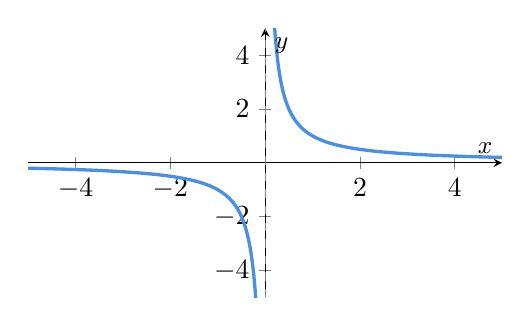
\begin{tikzpicture}\begin{axis}[width=7.6cm,height=5cm,axis lines=middle,xlabel={\small$x$},ylabel={\small$y$},xmin=-5,xmax=5,ymin=-5,ymax=5,samples=160,restrict y to domain=-6:6]\addplot[exblue,very thick,domain=-5:-0.18]{1/x};\addplot[exblue,very thick,domain=0.18:5]{1/x};\draw[dashed,gray] (axis cs:0,-5)--(axis cs:0,5);\end{axis}\end{tikzpicture}\end{center}
\end{example}

\begin{example}{ex3}{Example 4 --- Domain}
Domain of $y=\dfrac{1}{x+2}$?\soln \textbf{Step 1:} The domain of $y=\dfrac{1}{x+2}$ excludes every $x$ that makes the denominator zero: $x+2=0\Rightarrow x=-2$.

\textbf{Answer:} all real numbers except $-2$, i.e.\ $x\ne-2$ (and $x=-2$ is a vertical asymptote of $y=\dfrac{1}{x+2}$).
\end{example}

\begin{example}{ex4}{Example 5 --- Equal degrees}
Horizontal asymptote of $y=\dfrac{2x}{x-1}$?\soln \textbf{Step 1:} In $y=\dfrac{2x}{x-1}$ the numerator $2x$ has degree $1$ and the denominator $x-1$ has degree $1$ --- equal degrees.

\textbf{Step 2:} The HA of $y=\dfrac{2x}{x-1}$ is the ratio of the leading coefficients: $y=\dfrac21=2$. Check: at $x=1000$, $y=\dfrac{2000}{999}\approx2.002$.

\textbf{Answer:} $y=2$.
\end{example}

\begin{example}{ex5}{Example 6 --- A hole}
Describe $y=\dfrac{x^2-25}{x-5}$.\soln \textbf{Step 1 (factor):} The numerator of $y=\dfrac{x^2-25}{x-5}$ is a difference of squares: $x^2-25=(x-5)(x+5)$, so $y=\dfrac{(x-5)(x+5)}{x-5}$.

\textbf{Step 2 (cancel):} The factor $x-5$ cancels in $y=\dfrac{(x-5)(x+5)}{x-5}$, leaving $y=x+5$ for $x\ne5$.

\textbf{Step 3 (hole):} Substitute $x=5$ into the simplified $y=x+5$: $y=10$. The hole is at $(5,10)$, and there is no vertical asymptote at $x=5$ because the factor cancelled.

\textbf{Answer:} $y=\dfrac{x^2-25}{x-5}$ is the line $y=x+5$ with a hole at $(5,10)$.
\end{example}

\begin{example}{ex6}{Example 7 --- Shifted asymptote}
Vertical asymptote of $y=\dfrac{2}{x-4}$, graphed:\soln \textbf{Step 1:} Set the denominator of $y=\dfrac{2}{x-4}$ equal to zero: $x-4=0\Rightarrow x=4$. The numerator is $2\ne0$, so the VA is $x=4$ (dashed).

\textbf{Step 2:} In $y=\dfrac{2}{x-4}$ the numerator has degree $0<1$, so the HA is $y=0$ (dashed):\begin{center}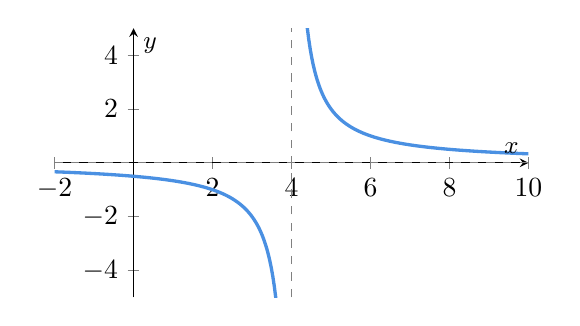
\begin{tikzpicture}\begin{axis}[width=7.6cm,height=5cm,axis lines=middle,xlabel={\small$x$},ylabel={\small$y$},xmin=-2,xmax=10,ymin=-5,ymax=5,samples=160,restrict y to domain=-6:6]\addplot[exblue,very thick,domain=-2:3.82]{2/(x-4)};\addplot[exblue,very thick,domain=4.18:10]{2/(x-4)};\draw[dashed,gray] (axis cs:4,-5)--(axis cs:4,5);\draw[dashed,gray] (axis cs:-2,0)--(axis cs:10,0);\end{axis}\end{tikzpicture}\end{center}
\end{example}

\begin{example}{ex7}{Example 8 --- Equal degrees}
Horizontal asymptote of $y=\dfrac{7x}{x-2}$?\soln \textbf{Step 1:} In $y=\dfrac{7x}{x-2}$ both the numerator $7x$ and the denominator $x-2$ have degree $1$.

\textbf{Step 2:} The HA of $y=\dfrac{7x}{x-2}$ is $y=\dfrac71=7$.

\textbf{Answer:} $y=7$ (the vertical asymptote of $y=\dfrac{7x}{x-2}$ is $x=2$).
\end{example}

\begin{example}{ex8}{Example 9 --- Domain}
Domain of $y=\dfrac{x}{x+7}$?\soln \textbf{Step 1:} The domain of $y=\dfrac{x}{x+7}$ excludes the $x$ that makes the denominator zero: $x+7=0\Rightarrow x=-7$.

\textbf{Step 2:} At $x=-7$ the numerator of $y=\dfrac{x}{x+7}$ is $-7\ne0$, so it is also a vertical asymptote.

\textbf{Answer:} $x\ne-7$.
\end{example}

\clearpage
\sech{Your Turn --- Show Your Work}
For each question, show all steps clearly in the space provided.

\begin{qbox}{Question 1}
Vertical asymptote of $y=\dfrac{1}{x-8}$?\workspace{2.4cm}
\end{qbox}

\begin{qbox}{Question 2}
Horizontal asymptote of $y=\dfrac{6}{x-2}$?\workspace{2.4cm}
\end{qbox}

\begin{qbox}{Question 3}
Domain of $y=\dfrac{x+3}{x-9}$?\workspace{2.4cm}
\end{qbox}

\begin{qbox}{Question 4}
Horizontal asymptote of $y=\dfrac{9x}{x-1}$?\workspace{2.4cm}
\end{qbox}

\begin{qbox}{Question 5}
Where is the hole in $y=\dfrac{x^2-49}{x-7}$?\workspace{2.4cm}
\end{qbox}

\begin{qbox}{Question 6}
Vertical asymptote of $y=\dfrac{2}{x+3}$?\workspace{2.4cm}
\end{qbox}

\begin{qbox}{Question 7}
Horizontal asymptote of $y=\dfrac{4x}{x-7}$?\workspace{2.4cm}
\end{qbox}

\begin{qbox}{Question 8}
Domain of $y=\dfrac{1}{x-1}$?\workspace{2.4cm}
\end{qbox}

\begin{qbox}{Question 9}
Horizontal asymptote of $y=\dfrac{1}{x^2+1}$?\workspace{2.4cm}
\end{qbox}

\begin{qbox}{Question 10}
Vertical asymptote of $y=\dfrac{x+1}{x-6}$?\workspace{2.4cm}
\end{qbox}

\begin{qbox}{Question 11}
Simplify $y=\dfrac{x^2-9}{x+3}$ and state any hole.\workspace{2.4cm}
\end{qbox}

\begin{qbox}{Question 12}
Horizontal asymptote of $y=\dfrac{3x}{2x-1}$?\workspace{2.4cm}
\end{qbox}

\begin{qbox}{Question 13 --- Challenge}
State the VA, HA and domain of $y=\dfrac{2x}{x-4}$.\workspace{3cm}
\end{qbox}

\clearpage
\sech{Question Recap \& Answer Key}

\begin{recapbox}
\begin{multicols}{2}
\small
\begin{enumerate}[leftmargin=*,itemsep=3pt]
  \item Vertical asymptote of $y=\dfrac{1}{x-8}$?
  \item Horizontal asymptote of $y=\dfrac{6}{x-2}$?
  \item Domain of $y=\dfrac{x+3}{x-9}$?
  \item Horizontal asymptote of $y=\dfrac{9x}{x-1}$?
  \item Where is the hole in $y=\dfrac{x^2-49}{x-7}$?
  \item Vertical asymptote of $y=\dfrac{2}{x+3}$?
  \item Horizontal asymptote of $y=\dfrac{4x}{x-7}$?
  \item Domain of $y=\dfrac{1}{x-1}$?
  \item Horizontal asymptote of $y=\dfrac{1}{x^2+1}$?
  \item Vertical asymptote of $y=\dfrac{x+1}{x-6}$?
  \item Simplify $y=\dfrac{x^2-9}{x+3}$ and state any hole.
  \item Horizontal asymptote of $y=\dfrac{3x}{2x-1}$?
  \item State the VA, HA and domain of $y=\dfrac{2x}{x-4}$.
\end{enumerate}
\end{multicols}
\end{recapbox}

\begin{keybox}
\begin{multicols}{2}
\small
\begin{enumerate}[leftmargin=*,itemsep=3pt]
  \item For $y=\dfrac{1}{x-8}$: $x-8=0\Rightarrow x=8$ (numerator $1\ne0$), so the VA is $x=8$
  \item For $y=\dfrac{6}{x-2}$: numerator degree $0<$ denominator degree $1$, so the HA is $y=0$
  \item For $y=\dfrac{x+3}{x-9}$: $x-9=0\Rightarrow x=9$ is excluded, so the domain is $x\ne9$
  \item For $y=\dfrac{9x}{x-1}$: equal degrees, $\dfrac91=9$, so the HA is $y=9$
  \item $y=\dfrac{x^2-49}{x-7}=\dfrac{(x-7)(x+7)}{x-7}=x+7$ for $x\ne7$; the hole is at $x=7$, i.e.\ $(7,14)$
  \item For $y=\dfrac{2}{x+3}$: $x+3=0\Rightarrow x=-3$ (numerator $2\ne0$), so the VA is $x=-3$
  \item For $y=\dfrac{4x}{x-7}$: equal degrees, $\dfrac41=4$, so the HA is $y=4$ (and the VA is $x=7$)
  \item For $y=\dfrac{1}{x-1}$: $x-1=0\Rightarrow x=1$ is excluded, so the domain is $x\ne1$
  \item For $y=\dfrac{1}{x^2+1}$: numerator degree $0<$ denominator degree $2$, so the HA is $y=0$ (and $x^2+1\ne0$, so there is no VA)
  \item For $y=\dfrac{x+1}{x-6}$: $x-6=0\Rightarrow x=6$ (numerator $6+1=7\ne0$), so the VA is $x=6$
  \item $y=\dfrac{x^2-9}{x+3}=\dfrac{(x-3)(x+3)}{x+3}=x-3$ for $x\ne-3$; the hole is at $x=-3$, i.e.\ $(-3,-6)$
  \item For $y=\dfrac{3x}{2x-1}$: equal degrees, $\dfrac32$, so the HA is $y=\tfrac32$ (and the VA is $x=\tfrac12$)
  \item For $y=\dfrac{2x}{x-4}$: VA $x-4=0\Rightarrow x=4$ (numerator $8\ne0$); HA equal degrees, $\dfrac21=2$, so $y=2$; domain $x\ne4$
\end{enumerate}
\end{multicols}
\end{keybox}

\end{document}
